%% ------- ROZDZIAŁ 4 ------- %%

\chapter{Testy aplikacji}

\section{Cel przeprowadzonych analiz}

Wykorzystując napisaną na potrzeby niniejszej pracy aplikację przeprowadzono testy, które zmierzają do porównania wybranych modeli regresji dostępnych w pakiecte \textit{Scikit-learn}.\\

Testy przeprowadzone zostały na dwóch zbiorach danych: cen giełdowych firmy Microsoft w zakresie od 2017-01-01 do 2017-10-30, oraz cen giełdowych firmy Intel w zakresie od 2017-01-01 do 2017-04-30.
W dlaszej części zbiory te będą nazywane odpowiednio: zbiór szeroki i zbiór wąski.
Dane wykorzystane do testów były cenami otwarcia.\\

Każdy przeprowadzony test uwzględnia wyliczenie dwóch wartości: średniego błędu kwadratowego oraz wyniku predycji.\\

Średni błąd kwadratowy liczony jest poprzez wykorzystanie funknji \textit{sklearn.metrics.mean\_squared\_error} z pakietu \textit{Scikit-learn}, a jego wartość w wypadku predykcji idealnej wynosi zero.
Wynik predykcji jest natomiast liczony poprzez wywołanie metody \textit{score()} obieku danego modelu regresji, a jego wartość zmierza do osiągnięcia 1.0 w przypadku idealnym.\\

Przeprowadzono osobne testy dla każdej z trzech wartości procentowych ilości danych uczących w stosunku do ilości danych testowych: 20\%, 50\% oraz 80\%.\\

Wybrane modele regresji to:
\begin{itemize}
 \item Regresja Liniowa
 \item Regresja Grzbietowa (KRR)
 \item Regresja Wektorów Nośnych (SVR)
 \item Regresja Procesu Gaussa (GPR)
\end{itemize}

Reasumując, dla każdej z metod regresji wykonano sześć testów.\\

Celem testów jest porównanie modeli regresji dostępnych w pakiecie \textit{Scikit-learn} i wyciągnięcie wniosków dotyczących:
\begin{itemize}
 \item dokładności predyckji modeli w zależności od ilości danych uczących oraz całkowitej ilości danych
 \item zdolności modeli do reprezentacji trendu
 \item wpływu zmiany ilości danych uczących na dopasowanie modeli
 \item wpływu całkowitej ilości danych na dopasowanie modeli
\end{itemize}

\section{Testy zbioru danych: Microsoft}

\subsection{Informacje ogólne}
Zakres danych użytych do testów wynosi 209 próbek, w przedziale dat od 2017-01-01 do 2017-10-30 z krokiem wynoszącym jeden dzień.\\

\begin{figure}[h!]
\centering
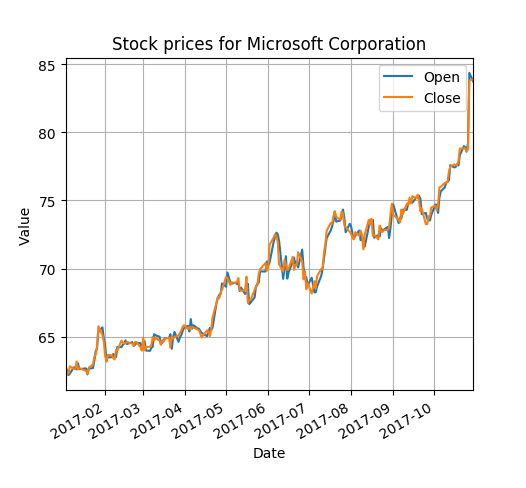
\includegraphics[width=150mm]{pictures/plots/microsoft_oc_price.png}
\caption{Wykres cen otwarcia i zamknięcia firmy Microsoft}
\label{fig:Wykres cen otwarcia i zamknięcia Microsoft}
\end{figure}

Na rysunku 4.1 przedstawiono wykres zmian cen otwarcia i zamknięcia dla podanego zakresu dat.\\ 

Ilość próbek danych uczących i testowych wynosi odpowiednio:
\begin{itemize}
 \item 41/168 dla wartości 20\% danych uczących
 \item 104/105 dla wartości 50\% danych uczących
 \item 167/42 dla wartości 80\% danych uczących
\end{itemize}
Na przedstawionych wykresach zaznaczona została linia podziału danych uczących i testowych i jest ona reprezentowana przez czerwoną pionową prostą.

\subsection{Regresja liniowa}
Wykres regresji liniowej dla podanego zbioru danych, przy proporcji 20\% danych uczących przedstawiony jest na rysunku 4.2.\\

\begin{figure}[h!]
\centering
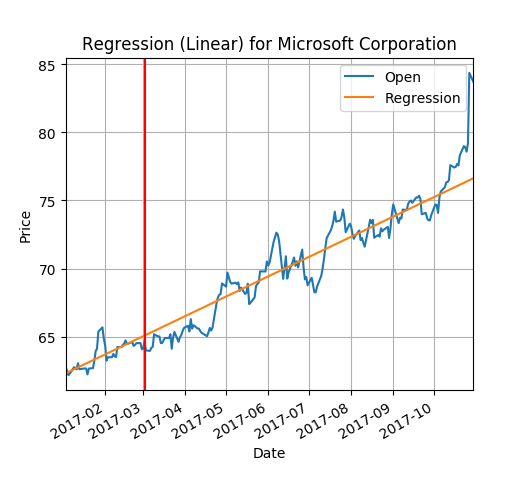
\includegraphics[width=150mm]{pictures/plots/microsoft_linear_20.png}
\caption{Wykres regresji liniowej dla 20\% danych uczących, Microsoft}
\label{fig:Wykres regresji liniowej dla 20\% danych uczących, Microsoft}
\end{figure}

Widoczny jest tu trend wzrostowy, który określony na podstawie danych uczących, kontunuowany jest także dla danych testowych.
Należy jednak zauważyć, że podany zbió© danych nie zawiera gwałtownych wzrostów i spadków cen w szczególności w części testowej, dzięki czemu regresja z powodzeniem przewiduje jego kontynuację.\\

Na rysunku 4.3 przedstawiono wykres regresji liniowej dla 50\% proporcji danych uczących.
\begin{figure}[h!]
\centering
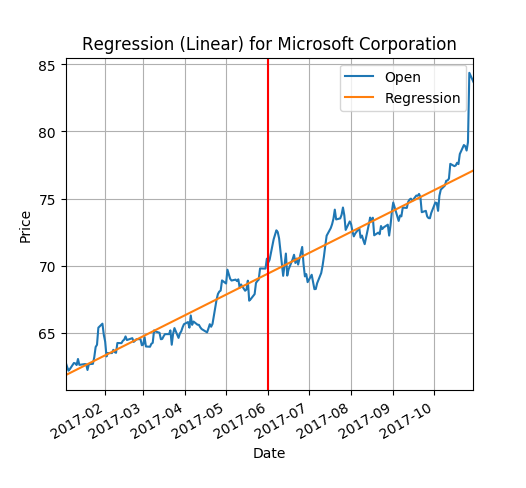
\includegraphics[width=150mm]{pictures/plots/microsoft_linear_50.png}
\caption{Wykres regresji liniowej dla 50\% danych uczących, Microsoft}
\label{fig:Wykres regresji liniowej dla 50\% danych uczących, Microsoft}
\end{figure}

Porównując wykresy 4.2 oraz 4.3 zauważalne jest niewielkie przesunięcie prostej regresji w kierunku niższej ceny, 
choć mimo tego można stwierdzić, że dla danego zbioru danych zwiększenie wartości podziału danych na testowe i uczące nie miało wpływu na wynik.

Rysunek 4.4 przedstawia wykres regresji liniowej dla 80\% proporcji danych uczących.\\

\begin{figure}[h!]
\centering
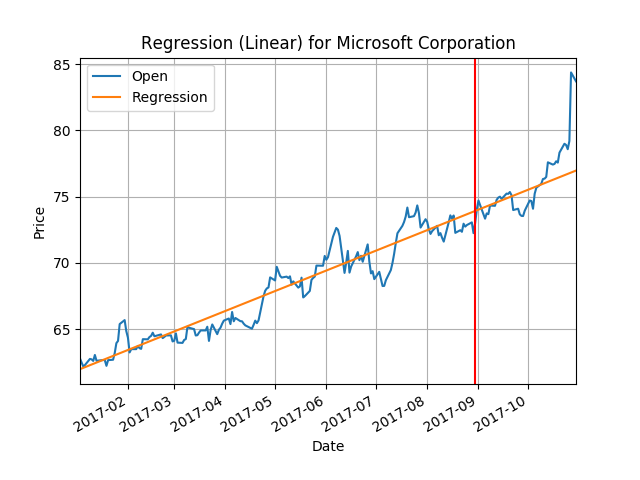
\includegraphics[width=150mm]{pictures/plots/microsoft_linear_80.png}
\caption{Wykres regresji liniowej dla 80\% danych uczących, Microsoft}
\label{fig:Wykres regresji liniowej dla 80\% danych uczących, Microsoft}
\end{figure}

W porównaniu do regresji liniowej przeprowadzonej dla 20\% i 50\% danych uczących, wyniki regresji przeprowadzonej dla 80\% danych uczących nie różnią się wiele od pozostałych.
Zauważalne jest jedynie delikatne przesunięcie prostej regresji w kierunku cen niższych, co może być spowodowane przez zmiany kierunku mniejszych trendów obecnych na wykresie.

\subsection{Regresja Grzbietowa}

\begin{figure}[h!]
\centering
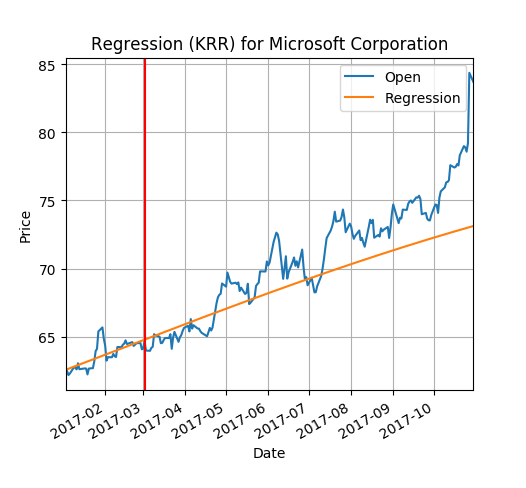
\includegraphics[width=150mm]{pictures/plots/microsoft_krr_20.png}
\caption{Wykres regresji grzbietowej dla 20\% danych uczących, Microsoft}
\label{fig:Wykres regresji grzbietowej dla 20\% danych uczących, Microsoft}
\end{figure}

\begin{figure}[h!]
\centering
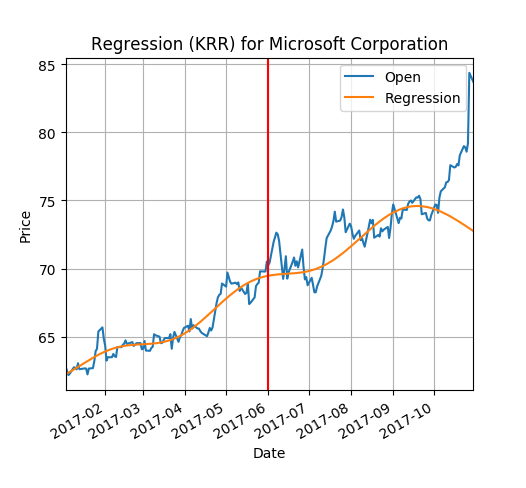
\includegraphics[width=150mm]{pictures/plots/microsoft_krr_50.png}
\caption{Wykres regresji grzbietowej dla 50\% danych uczących, Microsoft}
\label{fig:Wykres regresji grzbietowej dla 50\% danych uczących, Microsoft}
\end{figure}

\begin{figure}[h!]
\centering
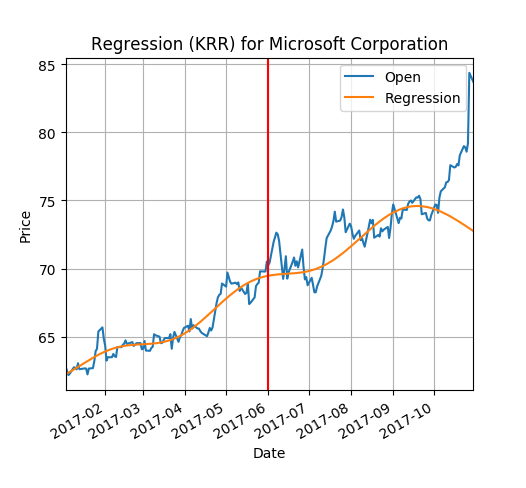
\includegraphics[width=150mm]{pictures/plots/microsoft_krr_50.png}
\caption{Wykres regresji grzbietowej dla 50\% danych uczących, Microsoft}
\label{fig:Wykres regresji grzbietowej dla 50\% danych uczących, Microsoft}
\end{figure}


\subsection{Regresja Wektorów Nośnych}

\begin{figure}[h!]
\centering
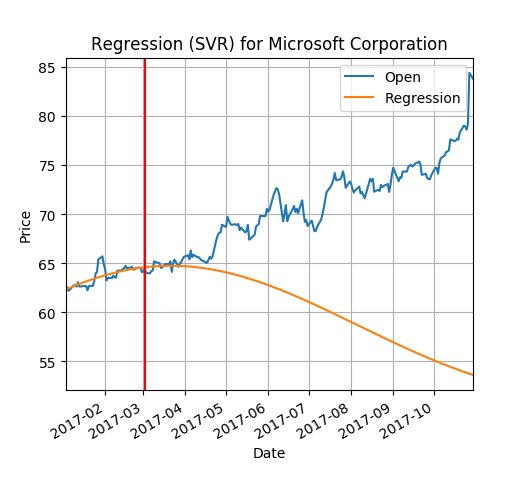
\includegraphics[width=150mm]{pictures/plots/microsoft_svr_20.png}
\caption{Wykres regresji wektorów nośnych dla 20\% danych uczących, Microsoft}
\label{fig:Wykres regresji wektorów nośnych dla 20\% danych uczących, Microsoft}
\end{figure}

\begin{figure}[h!]
\centering
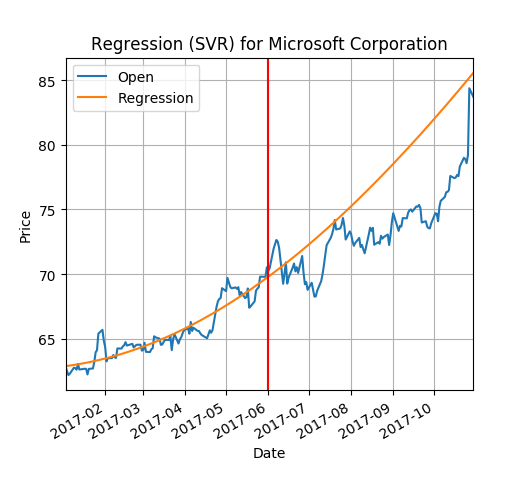
\includegraphics[width=150mm]{pictures/plots/microsoft_svr_50.png}
\caption{Wykres regresji wektorów nośnych dla 50\% danych uczących, Microsoft}
\label{fig:Wykres regresji wektorów nośnych dla 50\% danych uczących, Microsoft}
\end{figure}

\begin{figure}[h!]
\centering
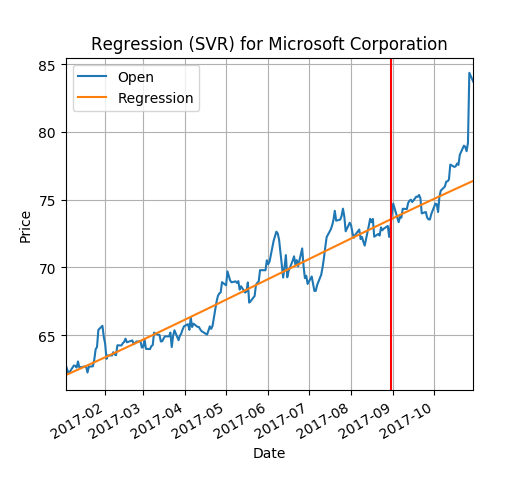
\includegraphics[width=150mm]{pictures/plots/microsoft_svr_80.png}
\caption{Wykres regresji wektorów nośnych dla 80\% danych uczących, Microsoft}
\label{fig:Wykres regresji wektorów nośnych dla 80\% danych uczących, Microsoft}
\end{figure}

\subsection{Regresja Procesu Gaussa}

\begin{figure}[h!]
\centering
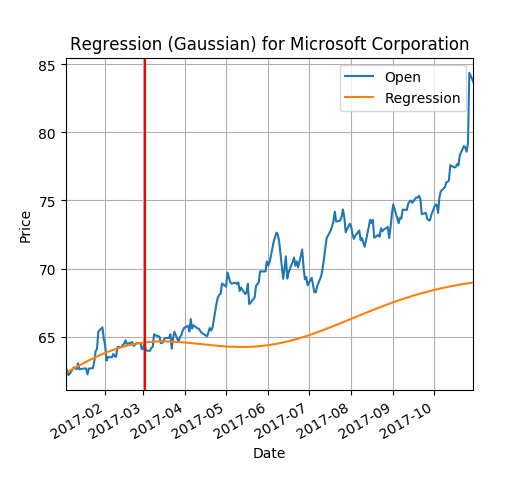
\includegraphics[width=150mm]{pictures/plots/microsoft_gpr_20.png}
\caption{Wykres regresji procesu Gaussa dla 20\% danych uczących, Microsoft}
\label{fig:Wykres regresji procesu Gaussa nośnych dla 20\% danych uczących, Microsoft}
\end{figure}

\begin{figure}[h!]
\centering
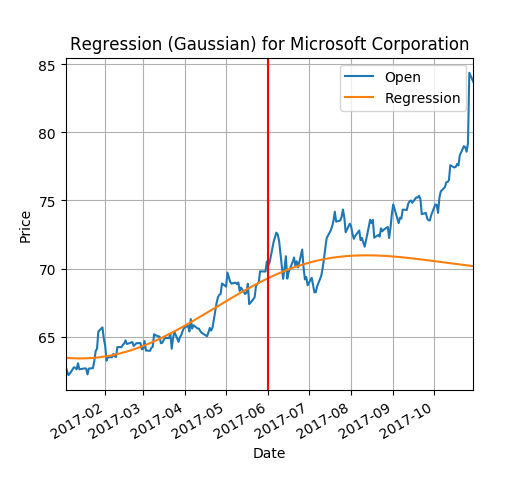
\includegraphics[width=150mm]{pictures/plots/microsoft_gpr_50.png}
\caption{Wykres regresji procesu Gaussa dla 50\% danych uczących, Microsoft}
\label{fig:Wykres regresji procesu Gaussa nośnych dla 50\% danych uczących, Microsoft}
\end{figure}

\begin{figure}[h!]
\centering
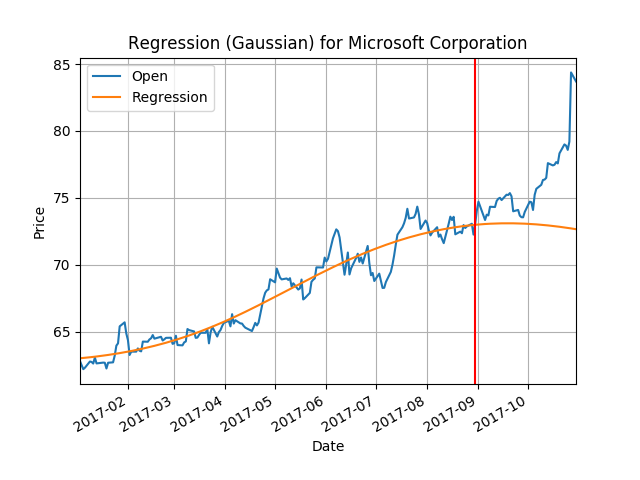
\includegraphics[width=150mm]{pictures/plots/microsoft_gpr_80.png}
\caption{Wykres regresji procesu Gaussa dla 80\% danych uczących, Microsoft}
\label{fig:Wykres regresji procesu Gaussa nośnych dla 80\% danych uczących, Microsoft}
\end{figure}

\subsection{Podsumowanie}

\begin{figure}[h!]
\centering
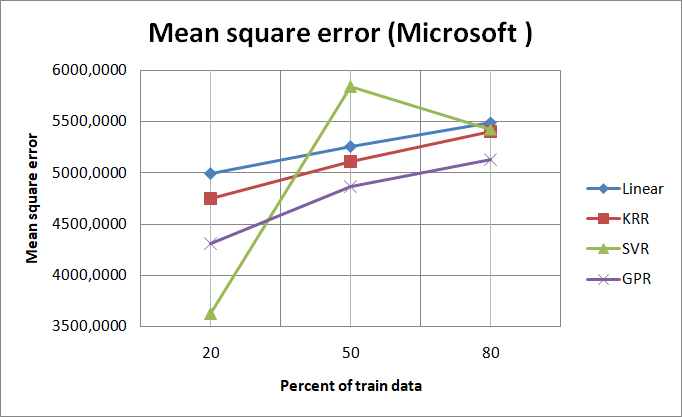
\includegraphics[width=150mm]{pictures/plots/microsoft_mean_square.png}
\caption{Wykres zmian wartości średniego błędu kwadratowego, Microsoft}
\label{fig:Wykres zmian wartości średniego błędu kwadratowego, Microsoft}
\end{figure}

\begin{figure}[h!]
\centering
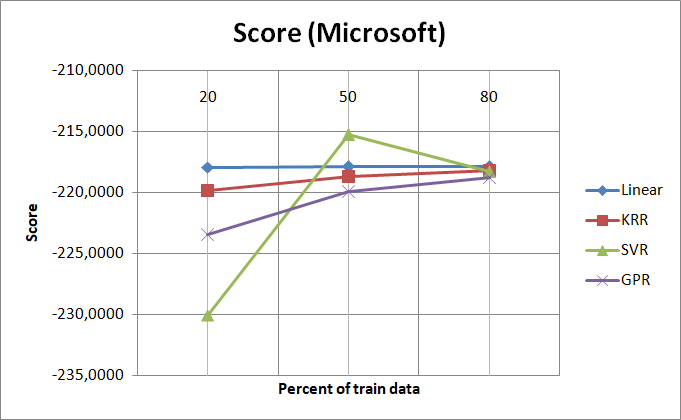
\includegraphics[width=150mm]{pictures/plots/microsoft_score.png}
\caption{Wykres zmian wartości wyników dopasowania modelu, Microsoft}
\label{fig:Wykres zmian wartości wyników dopasowania modelu, Microsoft}
\end{figure}



\section{Testy zbioru danych: Intel}

\subsection{Informacje ogólne}

\begin{figure}[h!]
\centering
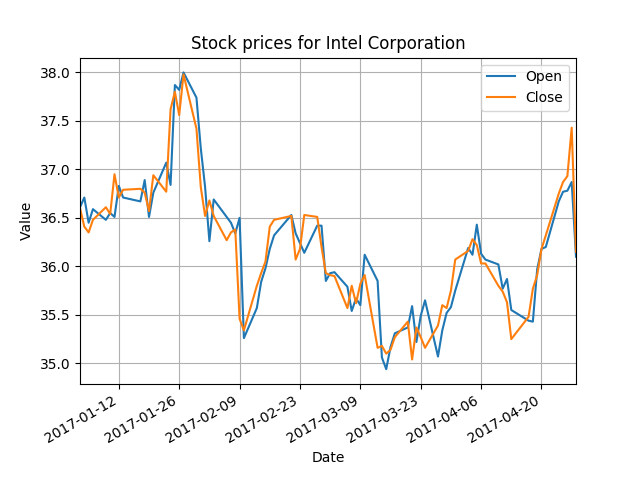
\includegraphics[width=150mm]{pictures/plots/intel_oc_price.png}
\caption{Wykres cen otwarcia i zamknięcia firmy Intel}
\label{fig:Wykres cen otwarcia i zamknięcia, Intel}
\end{figure}

\subsection{Regresja liniowa}

\begin{figure}[h!]
\centering
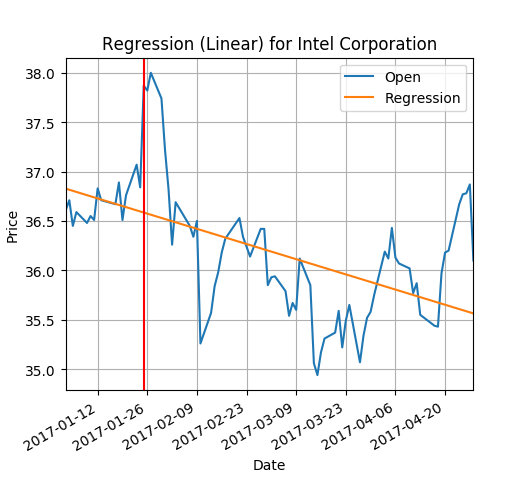
\includegraphics[width=150mm]{pictures/plots/intel_linear_20.png}
\caption{Wykres regresji liniowej dla 20\% danych uczących, Intel}
\label{fig:Wykres regresji liniowej dla 20\% danych uczących, Intel}
\end{figure}

\begin{figure}[h!]
\centering
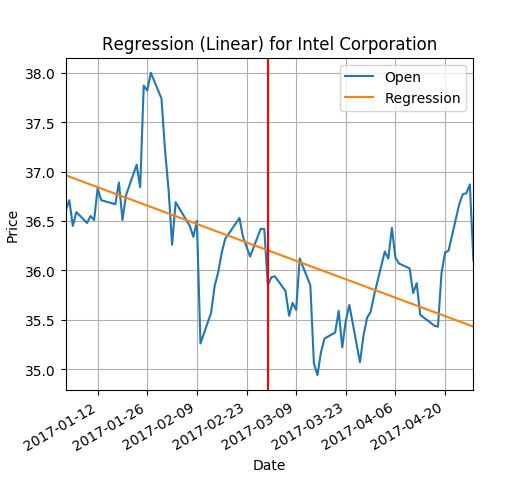
\includegraphics[width=150mm]{pictures/plots/intel_linear_50.png}
\caption{Wykres regresji liniowej dla 50\% danych uczących, Intel}
\label{fig:Wykres regresji liniowej dla 50\% danych uczących, Intel}
\end{figure}

\begin{figure}[h!]
\centering
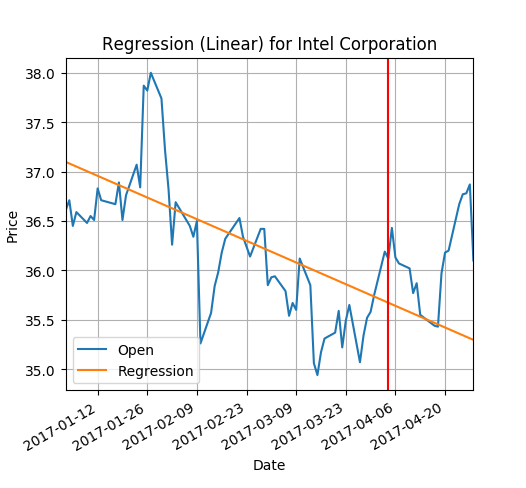
\includegraphics[width=150mm]{pictures/plots/intel_linear_80.png}
\caption{Wykres regresji liniowej dla 80\% danych uczących, Intel}
\label{fig:Wykres regresji liniowej dla 80\% danych uczących, Intel}
\end{figure}

\subsection{Regresja Grzbietowa}

\begin{figure}[h!]
\centering
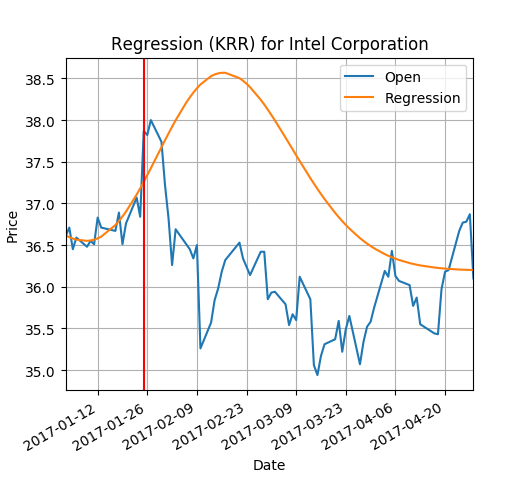
\includegraphics[width=150mm]{pictures/plots/intel_krr_20.png}
\caption{Wykres regresji grzbietowej dla 20\% danych uczących, Intel}
\label{fig:Wykres regresji grzbietowej dla 20\% danych uczących, Intel}
\end{figure}

\begin{figure}[h!]
\centering
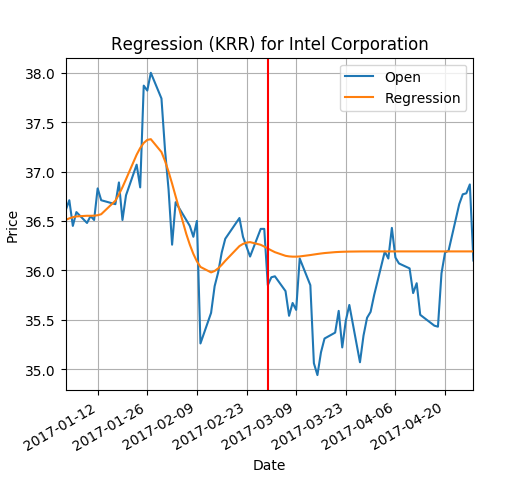
\includegraphics[width=150mm]{pictures/plots/intel_krr_50.png}
\caption{Wykres regresji grzbietowej dla 50\% danych uczących, Intel}
\label{fig:Wykres regresji grzbietowej dla 50\% danych uczących, Intel}
\end{figure}

\begin{figure}[h!]
\centering
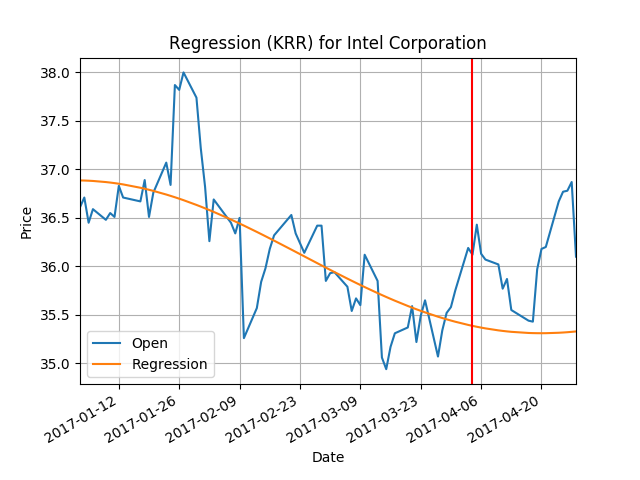
\includegraphics[width=150mm]{pictures/plots/intel_krr_80.png}
\caption{Wykres regresji grzbietowej dla 80\% danych uczących, Intel}
\label{fig:Wykres regresji grzbietowej dla 80\% danych uczących, Intel}
\end{figure}

\subsection{Regresja Wektorów Nośnych}

\begin{figure}[h!]
\centering
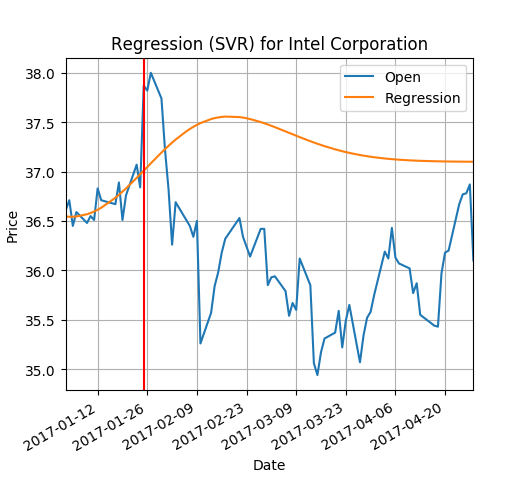
\includegraphics[width=150mm]{pictures/plots/intel_svr_20.png}
\caption{Wykres regresji wektorów nośnych dla 20\% danych uczących, Intel}
\label{fig:Wykres regresji wektorów nośnych dla 20\% danych uczących, Intel}
\end{figure}

\begin{figure}[h!]
\centering
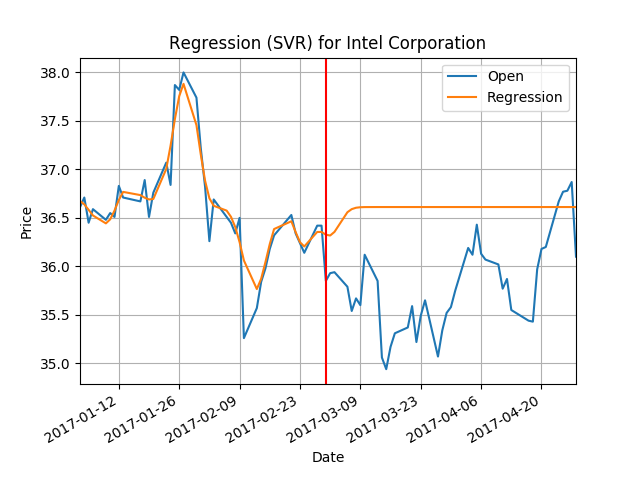
\includegraphics[width=150mm]{pictures/plots/intel_svr_50.png}
\caption{Wykres regresji wektorów nośnych dla 50\% danych uczących, Intel}
\label{fig:Wykres regresji wektorów nośnych dla 50\% danych uczących, Intel}
\end{figure}

\begin{figure}[h!]
\centering
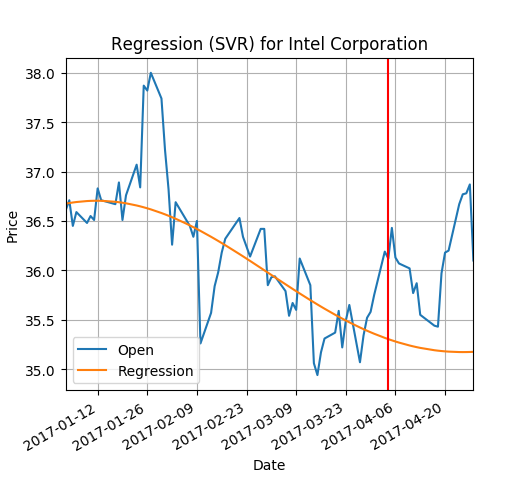
\includegraphics[width=150mm]{pictures/plots/intel_svr_80.png}
\caption{Wykres regresji wektorów nośnych dla 80\% danych uczących, Intel}
\label{fig:Wykres regresji wektorów nośnych dla 80\% danych uczących, Intel}
\end{figure}

\subsection{Regresja Procesu Gaussa}

\begin{figure}[h!]
\centering
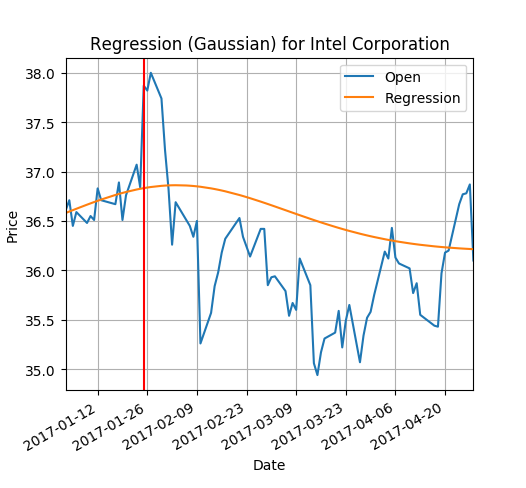
\includegraphics[width=150mm]{pictures/plots/intel_gpr_20.png}
\caption{Wykres regresji procesu Gaussa dla 20\% danych uczących, Intel}
\label{fig:Wykres regresji procesu Gaussa dla 20\% danych uczących, Intel}
\end{figure}

\begin{figure}[h!]
\centering
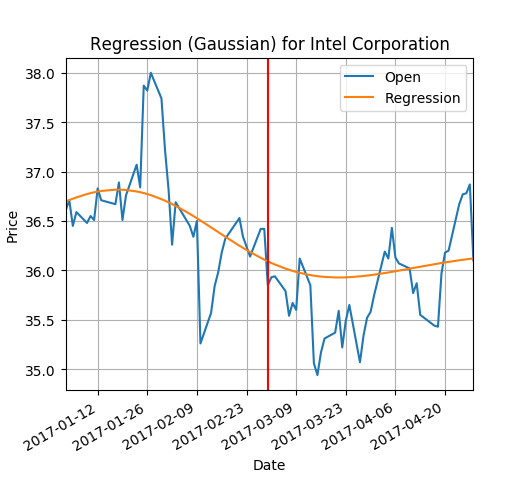
\includegraphics[width=150mm]{pictures/plots/intel_gpr_50.png}
\caption{Wykres regresji procesu Gaussa dla 50\% danych uczących, Intel}
\label{fig:Wykres regresji procesu Gaussa dla 50\% danych uczących, Intel}
\end{figure}

\begin{figure}[h!]
\centering
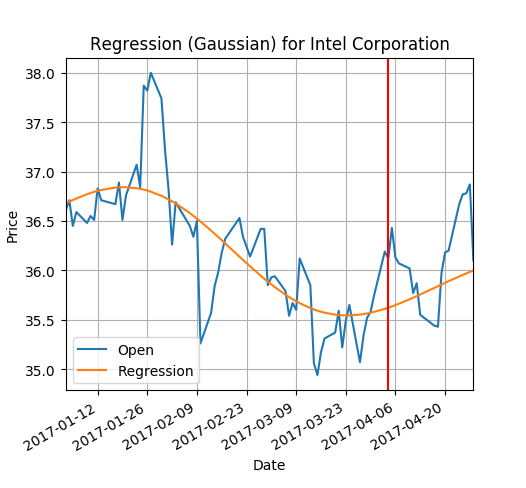
\includegraphics[width=150mm]{pictures/plots/intel_gpr_80.png}
\caption{Wykres regresji procesu Gaussa dla 80\% danych uczących, Intel}
\label{fig:Wykres regresji procesu Gaussa dla 80\% danych uczących, Intel}
\end{figure}

\subsection{Podsumowanie}

\begin{figure}[h!]
\centering
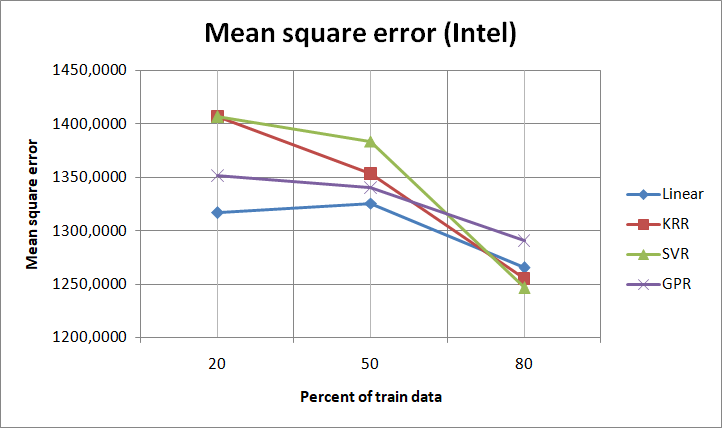
\includegraphics[width=150mm]{pictures/plots/intel_mean_square.png}
\caption{Wykres zmian wartości średniego błędu kwadratowego, Intel}
\label{fig:Wykres zmian wartości średniego błędu kwadratowego, Intel}
\end{figure}

\begin{figure}[h!]
\centering
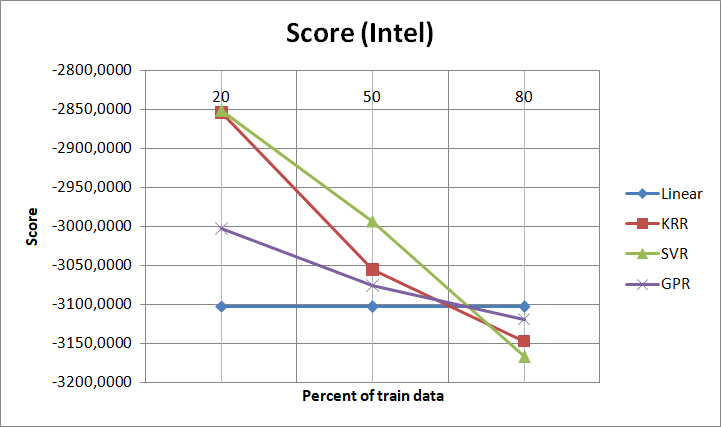
\includegraphics[width=150mm]{pictures/plots/intel_score.png}
\caption{Wykres zmian wartości wyników dopasowania modelu, Intel}
\label{fig:Wykres zmian wartości wyników dopasowania modelu, Intel}
\end{figure}

\section{Wnioski}
